% Options for packages loaded elsewhere
% Options for packages loaded elsewhere
\PassOptionsToPackage{unicode}{hyperref}
\PassOptionsToPackage{hyphens}{url}
\PassOptionsToPackage{dvipsnames,svgnames,x11names}{xcolor}
%
\documentclass[
  letterpaper,
  DIV=11,
  numbers=noendperiod]{scrartcl}
\usepackage{xcolor}
\usepackage{amsmath,amssymb}
\setcounter{secnumdepth}{-\maxdimen} % remove section numbering
\usepackage{iftex}
\ifPDFTeX
  \usepackage[T1]{fontenc}
  \usepackage[utf8]{inputenc}
  \usepackage{textcomp} % provide euro and other symbols
\else % if luatex or xetex
  \usepackage{unicode-math} % this also loads fontspec
  \defaultfontfeatures{Scale=MatchLowercase}
  \defaultfontfeatures[\rmfamily]{Ligatures=TeX,Scale=1}
\fi
\usepackage{lmodern}
\ifPDFTeX\else
  % xetex/luatex font selection
\fi
% Use upquote if available, for straight quotes in verbatim environments
\IfFileExists{upquote.sty}{\usepackage{upquote}}{}
\IfFileExists{microtype.sty}{% use microtype if available
  \usepackage[]{microtype}
  \UseMicrotypeSet[protrusion]{basicmath} % disable protrusion for tt fonts
}{}
\makeatletter
\@ifundefined{KOMAClassName}{% if non-KOMA class
  \IfFileExists{parskip.sty}{%
    \usepackage{parskip}
  }{% else
    \setlength{\parindent}{0pt}
    \setlength{\parskip}{6pt plus 2pt minus 1pt}}
}{% if KOMA class
  \KOMAoptions{parskip=half}}
\makeatother
% Make \paragraph and \subparagraph free-standing
\makeatletter
\ifx\paragraph\undefined\else
  \let\oldparagraph\paragraph
  \renewcommand{\paragraph}{
    \@ifstar
      \xxxParagraphStar
      \xxxParagraphNoStar
  }
  \newcommand{\xxxParagraphStar}[1]{\oldparagraph*{#1}\mbox{}}
  \newcommand{\xxxParagraphNoStar}[1]{\oldparagraph{#1}\mbox{}}
\fi
\ifx\subparagraph\undefined\else
  \let\oldsubparagraph\subparagraph
  \renewcommand{\subparagraph}{
    \@ifstar
      \xxxSubParagraphStar
      \xxxSubParagraphNoStar
  }
  \newcommand{\xxxSubParagraphStar}[1]{\oldsubparagraph*{#1}\mbox{}}
  \newcommand{\xxxSubParagraphNoStar}[1]{\oldsubparagraph{#1}\mbox{}}
\fi
\makeatother


\usepackage{longtable,booktabs,array}
\usepackage{calc} % for calculating minipage widths
% Correct order of tables after \paragraph or \subparagraph
\usepackage{etoolbox}
\makeatletter
\patchcmd\longtable{\par}{\if@noskipsec\mbox{}\fi\par}{}{}
\makeatother
% Allow footnotes in longtable head/foot
\IfFileExists{footnotehyper.sty}{\usepackage{footnotehyper}}{\usepackage{footnote}}
\makesavenoteenv{longtable}
\usepackage{graphicx}
\makeatletter
\newsavebox\pandoc@box
\newcommand*\pandocbounded[1]{% scales image to fit in text height/width
  \sbox\pandoc@box{#1}%
  \Gscale@div\@tempa{\textheight}{\dimexpr\ht\pandoc@box+\dp\pandoc@box\relax}%
  \Gscale@div\@tempb{\linewidth}{\wd\pandoc@box}%
  \ifdim\@tempb\p@<\@tempa\p@\let\@tempa\@tempb\fi% select the smaller of both
  \ifdim\@tempa\p@<\p@\scalebox{\@tempa}{\usebox\pandoc@box}%
  \else\usebox{\pandoc@box}%
  \fi%
}
% Set default figure placement to htbp
\def\fps@figure{htbp}
\makeatother





\setlength{\emergencystretch}{3em} % prevent overfull lines

\providecommand{\tightlist}{%
  \setlength{\itemsep}{0pt}\setlength{\parskip}{0pt}}



 


\KOMAoption{captions}{tableheading}
\makeatletter
\@ifpackageloaded{caption}{}{\usepackage{caption}}
\AtBeginDocument{%
\ifdefined\contentsname
  \renewcommand*\contentsname{Table of contents}
\else
  \newcommand\contentsname{Table of contents}
\fi
\ifdefined\listfigurename
  \renewcommand*\listfigurename{List of Figures}
\else
  \newcommand\listfigurename{List of Figures}
\fi
\ifdefined\listtablename
  \renewcommand*\listtablename{List of Tables}
\else
  \newcommand\listtablename{List of Tables}
\fi
\ifdefined\figurename
  \renewcommand*\figurename{Figure}
\else
  \newcommand\figurename{Figure}
\fi
\ifdefined\tablename
  \renewcommand*\tablename{Table}
\else
  \newcommand\tablename{Table}
\fi
}
\@ifpackageloaded{float}{}{\usepackage{float}}
\floatstyle{ruled}
\@ifundefined{c@chapter}{\newfloat{codelisting}{h}{lop}}{\newfloat{codelisting}{h}{lop}[chapter]}
\floatname{codelisting}{Listing}
\newcommand*\listoflistings{\listof{codelisting}{List of Listings}}
\makeatother
\makeatletter
\makeatother
\makeatletter
\@ifpackageloaded{caption}{}{\usepackage{caption}}
\@ifpackageloaded{subcaption}{}{\usepackage{subcaption}}
\makeatother
\usepackage{bookmark}
\IfFileExists{xurl.sty}{\usepackage{xurl}}{} % add URL line breaks if available
\urlstyle{same}
\hypersetup{
  pdftitle={Selection Bias \& Missing Data Challenge - Part 1},
  colorlinks=true,
  linkcolor={blue},
  filecolor={Maroon},
  citecolor={Blue},
  urlcolor={Blue},
  pdfcreator={LaTeX via pandoc}}


\title{Selection Bias \& Missing Data Challenge - Part 1}
\usepackage{etoolbox}
\makeatletter
\providecommand{\subtitle}[1]{% add subtitle to \maketitle
  \apptocmd{\@title}{\par {\large #1 \par}}{}{}
}
\makeatother
\subtitle{Blue Noise Stippling: Creating Art from Data}
\author{}
\date{}
\begin{document}
\maketitle


\subsection{The Problem: Can Algorithms Create
Art?}\label{the-problem-can-algorithms-create-art}

\textbf{Core Question:} How can we convert a photograph into an
aesthetically pleasing pattern of dots that preserves the visual
information of the original image?

\textbf{The Challenge:} Blue noise stippling is a technique that
converts images into patterns of dots (stipples) using algorithms that
balance visual accuracy with spatial distribution. This challenge asks
you to implement a modified ``void and cluster'' algorithm that combines
importance sampling with blue noise distribution properties to create
stippling patterns that are both visually accurate and spatially
well-distributed.

\textbf{Our Approach:} We'll use a modified void-and-cluster algorithm
that: 1. Creates an importance map identifying visually important
regions 2. Uses a toroidal (periodic) Gaussian kernel for repulsion to
ensure blue noise properties 3. Iteratively selects points with minimum
energy 4. Balances image content importance with blue noise spatial
distribution

\subsection{Introduction to Blue Noise
Stippling}\label{introduction-to-blue-noise-stippling}

Blue noise stippling is a technique for converting images into a pattern
of dots (stipples) that preserves the visual information of the original
image while creating an aesthetically pleasing, evenly distributed
pattern. This method follows the approach described by
\href{https://bartwronski.com/2022/08/31/progressive-image-stippling-and-greedy-blue-noise-importance-sampling/}{Bart
Wronski}.

The method uses a modified ``void and cluster'' algorithm that combines
importance sampling with blue noise distribution properties to create
stippling patterns that are both visually accurate and spatially
well-distributed. This version uses \textbf{smooth extreme
downweighting} that selectively downweights very dark and very light
tones while preserving mid-tones, creating a more balanced distribution
of stipples across the image.

\subsection{Loading the Original
Image}\label{loading-the-original-image}

First, let's load an image that we'll convert to a blue noise stippling
pattern. You can use any image you'd like, but we'll demonstrate with
the provided example.

\begin{figure}[H]

{\centering \pandocbounded{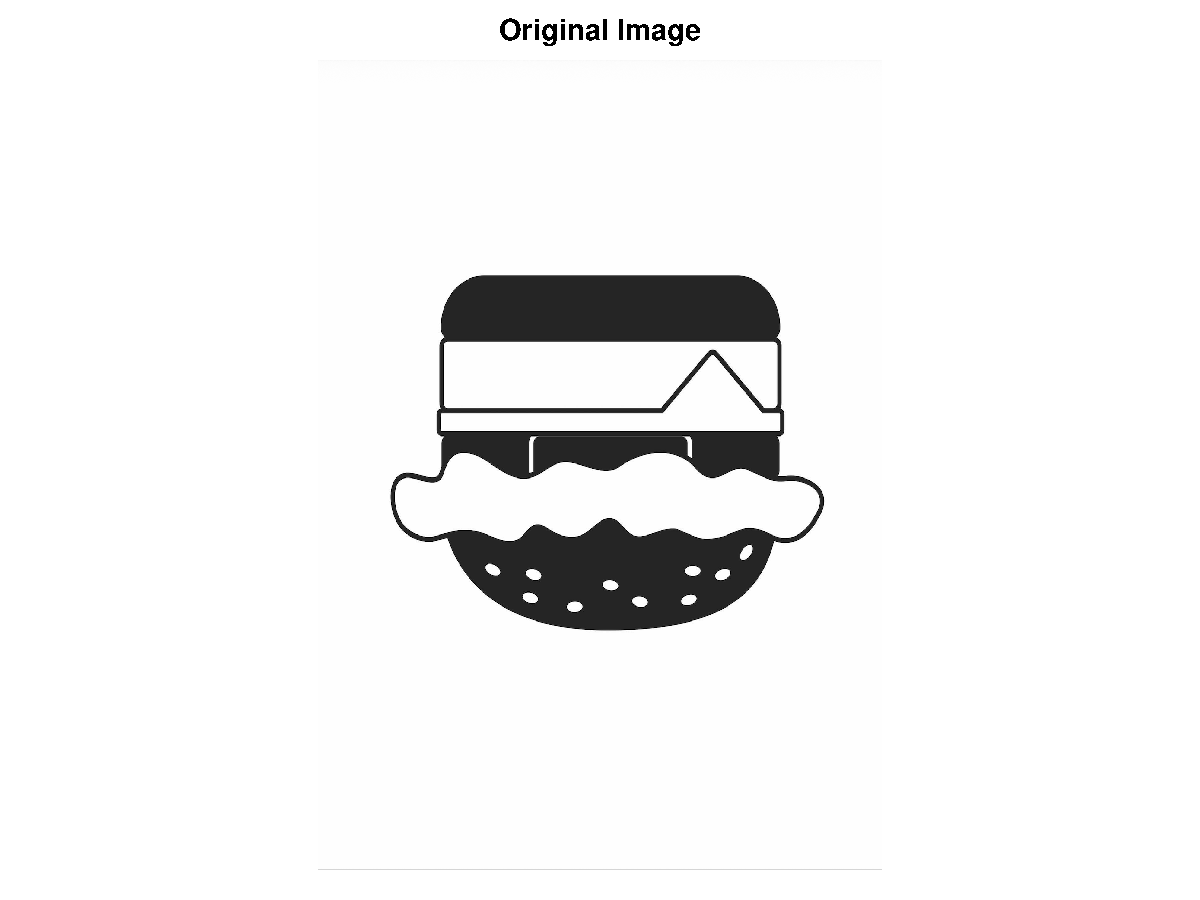
\includegraphics[keepaspectratio]{index_files/figure-pdf/load-image-r-1.pdf}}

}

\caption{Original image before stippling}

\end{figure}%

\begin{verbatim}
Image dimensions: 1564 x 1304 pixels
\end{verbatim}

\subsection{Importance Mapping}\label{importance-mapping}

Before applying the stippling algorithm, we create an \textbf{importance
map} that identifies which regions of the image should receive more
stipples. The importance map is computed by:

\begin{itemize}
\tightlist
\item
  \textbf{Brightness inversion}: The image brightness is inverted so
  that dark areas receive higher importance and thus more dots, while
  light areas receive fewer dots
\item
  \textbf{Extreme tone downweighting}: Smooth Gaussian functions
  downweight tones below 0.2 (very dark) and above 0.8 (very light),
  creating a gradual transition that preserves mid-tones
\item
  \textbf{Mid-tone boost}: A smooth Gaussian function centered on
  mid-tones provides a gradual increase in importance for mid-tone
  regions, ensuring they receive appropriate stippling density
\item
  \textbf{Selective and effective}: This approach ensures that stipples
  are distributed appropriately (more dots in dark areas and mid-tones,
  fewer in extreme dark/light areas) while maintaining good spatial
  distribution
\end{itemize}

\#\textbar{} label: importance-map-r \#\textbar{} echo: false
\#\textbar{} message: false \#\textbar{} warning: false

compute\_importance \textless- function(gray\_img, extreme\_downweight =
0.5, extreme\_threshold\_low = 0.4, extreme\_threshold\_high = 0.8,
extreme\_sigma = 0.1, mid\_tone\_boost = 0.4, mid\_tone\_sigma = 0.2) \{
\# Clip image to {[}0, 1{]} I \textless- pmax(pmin(gray\_img, 1.0), 0.0)

\# Invert brightness I\_inverted \textless- 1.0 - I

\# Dark mask \ldots{} (380 lines left)




\end{document}
